\chapter{Autovalores de Matrizes Simétricas com Algoritmos Genéticos\label{sec:metodo}}

	Os métodos que estudei para esta dissertação estão contidos em uma série de artigos \cite{metodo2002, metodo2004, metodo2006, metodo2008, metodo2009, metodo2011}. O objetivo é encontrar, sequencialmente, do menor para o maior, os autovalores de uma matriz simétrica. Essa matriz é o Hamiltoniano presente na formulação matricial da equação de Schrödinger independente do tempo\footnote{Ela é importante para a física moderna pois está associada à quantização da energia na Mecânica Quântica.}. A estratégia é transformar o problema do autovalor em um problema de otimização, buscando um escalar $a_i$ e um vetor $X_i$ de modo que a equaçaõ $HX_i = a_iX_i$ seja satisfeita.
	
	Os algoritmos apresentados em \cite{metodo2004} e \cite{metodo2011} são mais simples. Por exemplo, em \cite{metodo2002} o Hamiltoniano é alterado por algumas trasformações ortogonais e, só então, o \emph{fitness} é calculado. Nos artigos \cite{metodo2006}, \cite{metodo2008} e \cite{metodo2009} o espaço vetorial é dividido em duas partes de dimensões diferentes, levando a um Hamiltoniano que contém alguns autovalores de interesse\footnote{\emph{Partitioned matrix eigenvalue problem.}}. Isso não ocorre com os GAs das publicações de 2004 e 2011. Nelas o Hamiltoniano original é sempre mantido.
	
	Pode-se dizer que \cite{metodo2011} é a continuação de \cite{metodo2004}. A representação cromossomial e os operadores de seleção, \emph{crossover} e mutação são os mesmos. No entanto, ele adiciona dois operadores genéticos. O primeiro é complementar à mutação, e atua para criar mais diversidade na população. O segundo acentua a pressão seletiva via Elitismo. Não há justificativa para os novos operadores. Acredito que o intuito tenha sido melhorar a qualidade dos resultados, mas, infelizmente, não há comparação com os obtidos em 2004. E, de fato, isso seria impossível, pois em 2011 há uma mudança drástica: a função de avaliação foi alterada. Além disso, \cite{metodo2011} paraleliza o GA e compara os desempenhos.
	
	Assim, optei por seguir uma combinação entre \cite{metodo2004} e \cite{metodo2011}. Isso permitiu, por exemplo, comparar com segurança os resultados das duas funções de avaliação, algo que os autores não fizeram. A partir do próximo parágrafo descrevo o conteúdo dos dois artigos e como fiz a combinação entre os dois.

%========================================================	
%\section{Descrição do Algoritmo}
%========================================================	

	É possível expandir as soluções $\psi$ da Equação de Schrödinger independente do tempo em termos dos vetores geradores $\phi_k$ de uma base ortonormal finita $\phi$:
	
	\begin{equation}
		\psi = \sum_k c_k \phi_k.
	\end{equation}
	
	Isso leva ao problema de autovalores
	
	\begin{equation}\label{eq:HCEC}
		HC = EC,
	\end{equation}
	onde $H$ é uma matriz real e simétrica, construída na base ${\phi}$, que representa o operador Hamiltoniano. A diagonalização de $H$ encontra os autovalores $E_n$ correspondentes às energias possíveis do sistema quântico. Com isso, é possível obter os autovetores (autoestados) $C_n$ associados.
	
	No artigo \cite{metodo2004} é apresentada uma maneira de reduzir o problema de autovalores a um problema de busca. Dados todos os vetores $C$ existentes na base $\phi$, conjunto chamado de \textbf{Espaço de Busca}, o objetivo é encontrar os autovetores $C_n$ que satisfaçam a equação \ref{eq:HCEC}. O conjunto de todos os autovetores $C_n$ é o \textbf{Espaço de Soluções}. O mecanismo de busca é um algoritmo genético (GA).
	
	Conforme visto no capítulo \ref{cap:ga}, o elo entre o GA e o problema a ser resolvido está na Representação Cromossomial e na Função de Avaliação. O cromossomo deve codificar a solução desejada na forma de um \emph{string}, seja de caracteres, símbolos, números inteiros ou reais. O \emph{fitness} deve ser capaz de definir, objetivamente, a qualidade de todos os indivíduos da população, de modo que seja possível comparar cada um com as soluções desejadas. Quanto mais próximo um cromossomo está da solução, mais alto deve ser seu \emph{fitness}.

%-------------------------------------------------------		
	\section{Representação Cromossomial}
%-------------------------------------------------------	
	
	Como a solução pretendida é um autovetor, o cromossomo codifica um vetor. Cada indivíduo $i$ da população é um vetor $\psi_i$ candidato a autovetor na forma
	
	\begin{equation}
		\psi_i = \sum_{p=1}^m c_{pi}\phi_p, \mbox{   } i = 1,2, \cdots, n
	\end{equation}
	
	Na equação acima, $i$ varia de 1 até o número máximo de indivíduos na população do GA, mantida fixa ao longo de toda a execução. O índice $p$ é tomado de 1 até a $m$, que é ordem da matriz $H$ (ou a dimensão do espaço vetorial).
	
	O cromossomo é definido como uma cadeia de números reais, cujos valores são os coeficientes $c_{pi}$. O \emph{string} $S_i$, codificação para o membro $\psi_i$, é dado por
	
	\begin{equation}
		S_i \equiv  (c_{1i}, c_{2i}, \cdots, c_{pi}, \cdots, c_{mi}) = C^{\dagger}_i,
	\end{equation}
	enquanto que para outro membro $\psi_k$ da população, o \emph{string} $S_k$ é
	
	\begin{equation}
		S_k \equiv  (c_{1k}, c_{2k}, \cdots, c_{pk}, \cdots, c_{mk}) = C^{\dagger}_k.
	\end{equation}
	
%-------------------------------------------------------
	\section{População}
%-------------------------------------------------------

	A população inicial é gerada aleatoriamente. Não há nenhuma preferência com relação aos valores iniciais de cada gene.
	
	Seu tamanho (número de indivíduos) é sempre mantido fixo a cada nova geração.
	
%-------------------------------------------------------
	\section{Funções de Avaliação (\emph{fitness})}
	\label{sec:fitness_metodo}
%-------------------------------------------------------	

	O \emph{fitness} proposto em \cite{metodo2004} é obtido em três passos:
	
	\begin{enumerate}
		\item \label{item:passo1} Cálculo do quociente de Rayleigh $\rho_i$ associado ao $i-$ésimo indivíduo $C_i$;
		\item \label{item:passo2} Cálculo do gradiente de $\rho_i$;
		\item \label{item:passo3} Cálculo da função de avaliação.
	\end{enumerate}
	
	Retomando o capítulo \ref{cap:algebra}, o quociente de Rayleigh é dado por
	
	\begin{equation}\label{eq:rho-GA}
		\rho_i = \frac{C_i^\dagger H C_i}{C_i^\dagger C_i},
	\end{equation}
	e seu gradiente por
	
	\begin{equation}\label{eq:grad_rho_metodo}
		\nabla \rho_i = \frac{2[H - \rho_i]C_i}{C_i^\dagger C_i}.
	\end{equation}
		
	O \emph{fitness} é então definido como \footnote{
		No artigo \cite{metodo2004} a equação originalmente apresentada é $f_i = e^{-\beta (\nabla \rho_i)^{\nabla \rho_i}}$. Acredito que tenha sido um erro de digitação por dois motivos. O primeiro é que tal definição não leva, necessariamente, ao comportamento esperado: $f_i \rightarrow 1$ quando $\nabla \rho_i \rightarrow \textbf{0}$. Em segundo lugar, nos artigos \cite{metodo2006},  \cite{metodo2008} e \cite{metodo2009}, que seguem o mesmo método, a função de avaliação é definida como $f_i = e^{-\beta (\nabla \rho_i)^{\dagger} (\nabla \rho_i)}$. Portanto, segui com a definição de $f_i$ da equação \ref{eq:fitness_extenso}.}
	
	\begin{equation}\label{eq:fitness_extenso}
		f_i = e^{-\beta (\nabla \rho_i)^\dagger (\nabla \rho_i)}.
	\end{equation}
	
	Lembrando que o módulo de um vetor $V$ é dado por $|V| = \sqrt{V^{\dagger} V}$, a equação \ref{eq:fitness_extenso} fica
	
	\begin{equation}\label{eq:fitness_grad}
		f_i(\nabla \rho_i) = e^{-\beta |\nabla \rho_i|^2}.
	\end{equation}
			 
	A função de avaliação $f_i$ está limitada entre zero e um, $f_i$ = (0,1]. Se $|\nabla \rho_i|^2 \gg 1$, $f_i \rightarrow 0$, indicando que $C_i$ possui baixa qualidade, está longe da solução. Por outro lado, se $\nabla \rho_i \rightarrow \textbf{0} $, $f_i \rightarrow 1$, e $C_i$ é uma boa aproximação para um autovetor. O parâmetro $\beta$ é escolhido para não haver \emph{over flow} ou \emph{under flow} da função exponencial.
	
	De acordo com os autores, a equação \ref{eq:fitness_grad} leva ao autovalor mínimo. Se algum $C_i$, em algum momento, é o autovetor fundamental $C_0$, o $\nabla \rho$ é nulo. Eles afirmam que ``\textit{Claramente, $f_i \rightarrow 1$ quando $\nabla \rho_i \rightarrow 0$, sinalizando que a evolução atingiu o verdadeiro autovetor fundamental de $H$ em $C_i$}''\footnote{Tradução livre de ``\textit{Clearly, $f_i \rightarrow 1$, as $\nabla \rho_i \rightarrow 0$, signalling that the evolution has hit the true ground state eigenvector of $H$ in the vector $C_i$}''.}. 
	
	Uma vez que $C_0$ foi encontrado, o próximo passo é obter o autovalor $E_0$ associado. Na verdade ele já foi calculado, e é simplesmente o valor do quociente de Rayleigh para $C_i$:
	
	\begin{equation}
		\rho_0 = \frac{C_i^{\dagger} H C_i}{C_i^{\dagger} C_i} = E_0.
	\end{equation}
	
	Quando o algoritmo chega nesse estágio tem-se o par $(C_0,E_0)$.
	
	Como já dito anteriormente, a função de avaliação foi alterada em \cite{metodo2011}, e é dada por 
	
	\begin{equation}\label{eq:fitness_EL_metodo}
		f_i(\rho_i) = e^{-\beta(\rho_i - E_L)^2},
	\end{equation}
	onde $E_L$ é um limite inferior para o autovalor mínimo procurado.
	
	Ela compartilha algumas propriedades com a equação \ref{eq:fitness_grad}. Está limitada no conjunto $f_i(\rho) = (0,1]$ e, quanto maior seu valor, melhor a qualidade do indivíduo. O parâmetro $\beta$ tem exatamente a mesma função. A busca utilizando $f_i(\rho)$ também termina quando $f_i \rightarrow 1$. ``\emph{Se $\rho_i \rightarrow E_L$ durante a busca, $f_i \rightarrow 1$ e $C_i$ se aproxima do autovetor fundamental de $H$}''\footnote{Tradução livre de ``If $\rho_i \rightarrow E_L$ during the search, $f_i \rightarrow 1$ and $C_i$ approaches the ground eigenvector of $H$''.}. Novamente, como já temos $C_0$, o autovalor $E_0$ é simplesmente o $\rho_i$ já calculado.	O cálculo de $f_i(\rho)$ executa os passos \ref{item:passo1} e \ref{item:passo3} de $f_i(\nabla\rho)$.
				
		A não ser por acidente, a condição $f_i \rightarrow 1$ não é satisfeita logo na primeira população. É necessário evoluir os indivíduos por meio dos operadores genéticos de seleção, reprodução e mutação. Eles serão apresentados nas seções seguintes.

%-------------------------------------------------------
\section{Seleção}
%-------------------------------------------------------	

			O operador de seleção utilizado tanto em \cite{metodo2004} quanto em \cite{metodo2011} é o da Roleta, com fatias proporcionais aos valores do \emph{fitness} \cite{Linden2008}. Se a população possui $q$ indivíduos, a roleta é ``girada'' $q$ vezes, de modo a criar a nova população com os $q$ cromossomos selecionados.
			
			Entretanto, utilizei a seleção por Torneio pelos motivos apresentados na seção \ref{sec:torneio}. Mantive o tamanho da população fixa.
									
%-------------------------------------------------------
\section{Reprodução}
%-------------------------------------------------------

	A operação de reprodução ($crossover$) é aplicada na nova população após a Seleção. Há diferença entre os operadores de reprodução de \cite{metodo2004} e \cite{metodo2011}. Apresentarei ambos e, ao final, justificarei porque escolhi como base o segundo.

%----------------------------------------------------	
\subsection{\emph{Crossover} em \cite{metodo2004}}
%----------------------------------------------------	
	
	Suponha que tenham sido escolhidos, aleatoriamente, um par de cromossomos ($S_k$, $S_l$) dentre todos os $N$ indivíduos da população:
	
	\begin{equation}
		\begin{array}{l}
			S_k = (c_{k1}, c_{k2}, \cdots, c_{kn})	\\
			S_l = (c_{l1}, c_{l2}, \cdots, c_{ln})	
		\end{array}
	\end{equation}

	Em seguida, um inteiro $p$ é obtido, também aleatoriamente, entre 1 e $n - 1$ [p = [$1$, $n$)]. Lembre-se que $n$ é a ordem da matriz $H$ e, portanto, a quantidade de coeficientes no \emph{string} $S_i$. A função de $p$ é determinar em qual posição (\emph{locus}) do cromossomo acontecerá a alteração.
	
	O operador cria o novo par ($S^{'}_k$, $S^{'}_l$):
	
	\begin{equation}
		\begin{array}{l}
			S^{'}_k = (c_{k1}, c_{k2}, \cdots, c^{'}_{kp} c_{k,p+1}, \cdots, c_{kn})	\\
			S^{'}_l = (c_{l1}, c_{l2}, \cdots,  c^{'}_{lp} c_{l,p+1}, \cdots, c_{ln}),	\\
			
		\end{array}
	\end{equation}
	onde
	
	\begin{equation}
		\begin{array}{l}
			c^{'}_{kp} = f c_{kp} + (1 - f) c_{lp}     \\
			c^{'}_{lp} = (1 - f) c_{kp} + f c_{lp}.
		\end{array}
	\end{equation}
	
	O parâmetro $f$ faz o papel da mistura que cria nova informação. Ele é gerado aleatoriamente com valores entre zero e um. Nesse caso os valores limite não estão inclusos [f = (0,1)]. Dessa maneira há garantia de mistura.
	
	Esse operador só age em uma certa fração da população, dada por uma probabilidade $p_c$ que, em geral, é grande (70$-$75\%). O restante da população não é alterado.

%-----------------
\textbf{Exemplo}
%-----------------

Na figura \ref{fig:cross2004_tabelaAntes} há dois cromossomos de tamanho $n = 6$. A posição onde ocorrerá a alteração dos valores foi obtida aleatoriamente entre $p = [1,6)$, e, para esse caso, vale $p = 4$. O valor de $S_k$ na posição $p = 4$ é $c_{k4} = 0,80$, e para $S_l$ é $c_{l4} = 0,39$. Para $p + 1$ os valores são $c_{k5} = 0,15$ e $c_{l5} = 0,89$.

\begin{figure}[htbp]
	\centering
		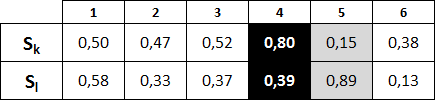
\includegraphics[width=0.70\textwidth]{figs/materiais_metodo/autovalores_com_ga/cross2004_tabelaAntes.png}
	\caption{Exemplo do \emph{crossover} de \cite{metodo2004}. Indivíduos antes da reprodução.}
	\label{fig:cross2004_tabelaAntes}
\end{figure}

O parâmetro $f$ teve seu valor determinado aleatoriamente como $f = 0,62$. Os valores de $c^{'}_{k4}$ e $c^{'}_{l4}$ ficam:

\begin{equation}\label{eq:ck4}
	\begin{array}{lccl}
		c^{'}_{kp} = & f c_{kp} & + & (1 - f) c_{lp} 						\\
		c^{'}_{k4} = & 0,62 c_{k4} & + & (1 - 0,62) c_{l4} 			\\
		c^{'}_{k4} = & 0,62 * 0,80 & + & 0,38 * 0,39 						\\		
		c^{'}_{k4} = & 0,496 & + & 0,1482	\\		
		c^{'}_{k4} = & 0,6442 &  & 
	\end{array}
\end{equation}

\begin{equation}\label{eq:cl4}
	\begin{array}{lccl}
		c^{'}_{lp} = & (1-f) c_{kp} & + & f c_{lp} 						\\
		c^{'}_{l4} = & (1-0,62) c_{k4} & + & 0,62 c_{l4} 						\\
		c^{'}_{l4} = & 0,38 * 0,80 & + & 0,62 * 0,39 						\\
		c^{'}_{l4} = & 0,304 & + & 0,2418 						\\
		c^{'}_{l4} = & 0,5458 &  & 
	\end{array}
\end{equation}

Finalmente, os valores para a posição $p = 4$ nos novos indivíduos $S^{'}_k$ e $S^{'}_l$ são

\begin{equation}\label{eq:cross2004_novo_valor_sk}
	\begin{array}{ll}
	\mbox{Novo valor na posição 4 de  } S^{'}_k & = c^{'}_{kp} c_{k,p+1} \\
								& = c^{'}_{k4} c_{k5} \\
								& = 0,6442 * 0,15	\\
								& = 0,09663	\\
								& \approx 0,1
	\end{array}
\end{equation}

\begin{equation}\label{eq:cross2004_novo_valor_sl}
	\begin{array}{ll}
	\mbox{Novo valor na posição 4 de  } S^{'}_l & = c^{'}_{lp} c_{l,p+1} \\
								& = c^{'}_{l4} c_{l5} \\
								& = 0,5458 * 0,89	\\
								& = 0,485762 \\
								& \approx  0,49
	\end{array}
\end{equation}


Na figura \ref{fig:cross2004_tabelaDepois} há os dois novos indivíduos.

\begin{figure}[htbp]
	\centering
		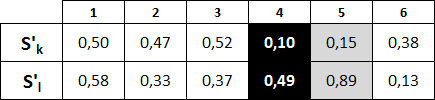
\includegraphics[width=0.70\textwidth]{figs/materiais_metodo/autovalores_com_ga/cross2004_tabelaDepois.png}
	\caption{Exemplo do \emph{crossover} de \cite{metodo2004}. Indivíduos depois da reprodução.}
	\label{fig:cross2004_tabelaDepois}
\end{figure}

%----------------------------------------------------
\subsection{\emph{Crossover} em \cite{metodo2011}}	
%----------------------------------------------------

	A representação cromossomial usada em \cite{metodo2011} é a mesma de \cite{metodo2004}, portanto, o par ($S_k$, $S_l$) é igual, assim como a probabilidade $p_c$:
	
	\begin{equation}
		\begin{array}{l}
		S_k = (c_{k1}, c_{k2}, \cdots, c_{kn})	\\
		S_l = (c_{l1}, c_{l2}, \cdots, c_{ln})	
		\end{array}
	\end{equation}
	
	Diferentemente de \cite{metodo2004}, utiliza-se o \emph{crossover} de dois pontos. Aleatoriamente escolhe-se dois inteiros, $o$ e $p$, cuja função é determinar a região do cromossomo que sofrerá miscigenação. O valor em $o$ indica o primeiro gene, e $p$ o último. Portanto, todos os genes entre os dois, incluindo eles próprios, sofrerão a ação do \emph{crossover} ($o <= c_i <= p$, $p \geq o$). Os novos indivíduos são ($S^{'}_k$, $^{'}S_l$)
	
	\begin{equation}
		\begin{array}{l}
			S^{'}_k = (c_{k1}, c_{k2}, \cdots, c^{'}_{ko}, \cdots , c^{'}_{kp}, c_{k,p+1}, \cdots, c_{kn})	\\
			S^{'}_l = (c_{l1}, c_{l2}, \cdots, c^{'}_{lo}, \cdots , c^{'}_{lp}, c_{l,p+1}, \cdots, c_{ln}).	
		\end{array}
	\end{equation}
	
	Para todos genes selecionados, a transformação ocorre da seguinte maneira ($i = o, o + 1, \cdots, p$):
	
	\begin{equation}
		\begin{array}{l}
			c^{'}_{ki} = f_c c_{ki} + (1 - f_c) c_{li}     \\
			c^{'}_{li} = (1 - f_c) c_{ki} + f_c c_{li}
		\end{array}
	\end{equation}
	onde $f_c$ é dado por
	
	\begin{equation}
		f_c = 0,75 + 0,25r,
	\end{equation}
	sendo $r$ um número aleatório ($0 \leq r \leq 1$). Assim como o parâmetro $f$ de \cite{metodo2004}, $f_c$ faz o papel da mistura que cria nova informação.
	
	\textbf{Exemplo}.
	
	
	Usei os mesmos indivíduos da figura \ref{fig:cross2004_tabelaAntes}. Os parâmetros $o$ e $p$ foram escolhidos no intervalo [1,6] e têm valores $o = 2$ e $p = 4$. Portanto, no \emph{string} $S_k$ os elementos que sofrerão alteração são $c_{k2} = 0,47$, $c_{k3} = 0,52$ e $c_{k4} = 0,80$. Eles se misturarão com os elementos $c_{l2} = 0,33$, $c_{l3} = 0,37$ e $c_{l4} = 0,39$ de $S_l$. Aleatoriamente obtive $r = 0,2$, que leva a $f_c = 0,80$.
	
	\begin{figure}[htbp]
	\centering
		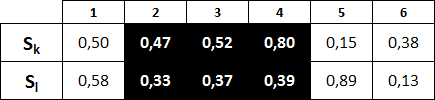
\includegraphics[width=0.70\textwidth]{figs/materiais_metodo/autovalores_com_ga/cross2011_tabelaAntes.png}
	\caption{Exemplo do \emph{crossover} de \cite{metodo2011}. Indivíduos antes da reprodução.}
	\label{fig:cross2011_tabelaAntes}
\end{figure}
	
	Os elementos $c^{'}_{ki}$ são:
	
	\begin{equation}
		\begin{array}{llcl}
			c^{'}_{k2}	& = f_c c_{k2} 		& + & (1- f_c) c_{l2} \\
									& = 0,80 * 0,47		& + &	(1 - 0,80) * 0,33 \\
									& = 0,376					& + & 0,2 * 0,33	\\
									& = 0,376					& + & 0,066	\\
									& = 0,442 \\
									& \approx 0,44
		\end{array}
	\end{equation}
	
	
	\begin{equation}
		\begin{array}{llcl}
			c^{'}_{k3}	& = f_c c_{k3} 		& + & (1- f_c) c_{l3} \\
									& = 0,80 * 0,52		& + &	(1 - 0,80) * 0,37 \\
									& = 0,416					& + & 0,2 * 0,37	\\
									& = 0,416					& + & 0,074	\\
									& = 0,49
		\end{array}
	\end{equation}
	
	
	\begin{equation}
		\begin{array}{llcl}
			c^{'}_{k4}	& = f_c c_{k4} 		& + & (1- f_c) c_{l4} \\
									& = 0,80 * 0,80		& + &	(1 - 0,80) * 0,39 \\
									& = 0,64					& + & 0,2 * 0,39	\\
									& = 0,64					& + & 0,078	\\
									& = 0,718 \\
									& \approx 0,72
		\end{array}
	\end{equation}
	
	
	Os elementos $c^{'}_{li}$ são:
	
	\begin{equation}
		\begin{array}{llcl}
			c^{'}_{l2}	& = (1 - f_c) c_{k2} 		& + & f_c c_{l2} \\
									& = (1 - 0,80) * 0,47		& + &	0,80 * 0,33 \\
									& = 0,2 * 0,47					& + & 0,264	\\
									& = 0,094					& + & 0,264	\\
									& = 0,358 \\
									& \approx 0,36
		\end{array}
	\end{equation}
	
	\begin{equation}
		\begin{array}{llcl}
			c^{'}_{l3}	& = (1 - f_c) c_{k3} 		& + & f_c c_{l3} \\
									& = (1 - 0,80) * 0,52		& + &	0,80 * 0,37 \\
									& = 0,2 * 0,52					& + & 0,296	\\
									& = 0,104								& + & 0,296	\\
									& = 0,40									
		\end{array}
	\end{equation}
	
	
	\begin{equation}
		\begin{array}{llcl}
			c^{'}_{l4}	& = (1 - f_c) c_{k4} 		& + & f_c c_{l4} \\
									& = (1 - 0,80) * 0,80		& + &	0,80 * 0,39 \\
									& = 0,2 * 0,80					& + & 0,312	\\
									& = 0,16								& + & 0,312	\\
									& = 0,472 \\
									& \approx 0,47
		\end{array}
	\end{equation}
	
	Os novos indivíduos estão na figura \ref{fig:cross2011_tabelaDepois}.
		
	\begin{figure}[htbp]
	\centering
		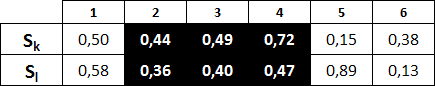
\includegraphics[width=0.70\textwidth]{figs/materiais_metodo/autovalores_com_ga/cross2011_tabelaDepois.png}
	\caption{Exemplo do \emph{crossover} de \cite{metodo2011}. Indivíduos depois da reprodução.}
	\label{fig:cross2011_tabelaDepois}
\end{figure}
	
	
%----------------------------------------------------
\subsection{\emph{Crossover} utilizado}
\label{sec:crossover_utilizado}
%----------------------------------------------------

	A quantidade de nova informação não é escalável com o tamanho do cromossomo no \emph{crossover} de \cite{metodo2004}. Ele altera apenas uma posição (locus) de cada indivíduo, independentemente do tamanho do cromossomo. Por exemplo, se a ordem do Hamiltoniano for $n = 100$, o \emph{string} terá 100 elementos, mas apenas um sofrerá alteração. O mesmo aconteceria para $n = 1.000$, 10.000 e assim por diante.
	
	Ainda sobre o artigo de 2004, é impossível haver troca de informação na última posição. O parâmetro $p$, obtido aleatoriamente, dá a posição na qual ocorrerá o \emph{crossover}. Porém, parte do cálculo envolve os elementos $c_{k,p+1}$ e $c_{l,p+1}$. Note o índice $p+1$. Como a posição máxima é $n$, o maior índice possível para estes elementos é $p + 1 = n$, impondo o limite $p \leq n - 1$. Nos exemplos apresentados, $n = 6$, $p \leq 5$ e, portanto, a posição $6$ nunca será escolhida.
	
	Isso pode dificultar a busca. Suponha que uma solução precise do valor 23 no último coeficiente do cromossomo ($c_n = 0,23$). Se nenhum indivíduo da população inicial já tiver nascido com ele, esse valor nunca aparecerá por meio do \emph{crossover}. Resta como esperança a Mutação, porém, por definição, ela tem baixa probabilidade \cite{Linden2008}. Também não há garantia de que, após muitas gerações com sucessivas operações de \emph{crossover}, mutação e seleção, haverá um indivíduo na população que, além de ter 0,23 na última posição, possua os outros $(n-1)$ primeiros elementos necessários.
		
		O \emph{crossover} de \cite{metodo2004} é um caso especial do \emph{crossover} de \cite{metodo2011}. O operador de reprodução de \cite{metodo2011} é o clássico \emph{crossover} de dois pontos \cite{Linden2008}. Nele, $p \geq o$, e, se $o = p$, há mistura em apenas uma posição do \emph{string}, exatamente o que acontece em \cite{metodo2004}. Como $1 \leq o \leq n$ e $1 \leq p \leq n$, o último gene também está sujeito à operação, e o problema citado no parágrafo anterior não existe.
		
	Pelo que expus acima, escolhi utilizar o \emph{crossover} de \cite{metodo2011}, mas com uma pequena modificação. No cálculo dos novos coeficientes $c^{'}_{i}$, em vez do parâmetro $f_c$, usei o $f$ conforme definido em \cite{metodo2004}. O $f$ pode variar entre $0$ e $1$, enquanto o $f_c$, além de necessitar do parâmetro adicional $r$, é limitado apenas entre $0,75$ e $1$. Assim, acredito que $f$ seja mais abrangente como parâmetro de mistura e criação de nova informação.
	
	\textbf{\emph{Crossover} utilizado}
	
	A seguir apresento sinteticamente a estrutura do \emph{crossover} utilizado. Um par de indivíduos $(S_k, S_l)$
	
	\begin{equation}
		\begin{array}{l}
			S_k = (c_{k1}, c_{k2}, \cdots, c_{kn})	\\
			S_l = (c_{l1}, c_{l2}, \cdots, c_{ln})	
		\end{array}
	\end{equation}
	é obtido aleatoriamente da população. Com probabilidade $p_c$, a operação de \emph{crossover} acontece. Dois pontos de corte $o$ e $p$ são obtidos, também aleatoriamente, gerando os novos \emph{strings} $S^{'}_k$ e $S^{'}_l$ na forma
		
	\begin{equation}
		\begin{array}{l}
			S^{'}_k = (c_{k1}, c_{k2}, \cdots, c^{'}_{ko}, \cdots , c^{'}_{kp}, c_{k,p+1}, \cdots, c_{kn})	\\
			S^{'}_l = (c_{l1}, c_{l2}, \cdots, c^{'}_{lo}, \cdots , c^{'}_{lp}, c_{l,p+1}, \cdots, c_{ln}),
		\end{array}
	\end{equation}
	onde
	
	\begin{equation}\label{eq:recombinacao}
		\begin{array}{l}
			c^{'}_{ki} = f c_{ki} + (1 - f) c_{li}     \\
			c^{'}_{li} = (1 - f) c_{ki} + f c_{li}
		\end{array}
	\end{equation}
	e
	
	\begin{equation}
	0 \leq f \leq 1 \mbox{       (obtido aleatoriamente)}
	\end{equation}

%-------------------------------------------------------
\section{Mutação}
%-------------------------------------------------------

	O operador Mutação é semelhante nos dois artigos. Todos os cromossomos estão sujeitos à mutação. Se um indivíduo $k$ sofre mutação no gene $q$, o antigo valor $c^{'}_{kq}$ é alterado para $c^{''}_{kq}$ com a seguinte equação:

		\begin{equation}\label{eq:mutacao}
			c^{''}_{kq} = c^{'}_{kq} + (-1)^{L} r \Delta,
		\end{equation}
		onde $L$ é um número inteiro, $r$ um número aleatório ($0 \leq r \leq 1$) e $\Delta$ é a intensidade da mutação.
		
		
	Não ficou claro para mim qual a relação entre a probabilidade $p_m$ e como será a mutação no artigo \cite{metodo2004}. Os autores dizem que todos os \emph{indivíduos} estão sujeitos ao operador, mas não citam quais \emph{genes} podem sofrer mutação. Essa informação está explícita em \cite{metodo2011}, que permite mutação, caso aconteça, em apenas um gene de cada indivíduo. Ou seja, se houver mutação logo no primeiro gene de um cromossomo, o algoritmo parte para o próximo indivíduo.
	
	Assumi que no artigo \cite{metodo2004} os autores utilizaram o operador clássico. Conforme a literatura \cite{Mitchell98, Linden2008} o operador clássico de mutação age com probabilidade $p_m$ em cada gene, de maneira individual e independente. Ou seja, se um gene $c_{k,j}$ sofreu ou não mutação, essa informação não é utilizada para avaliar a ocorrência de mutação no próximo gene $c_{k,j+1}$. Portanto, a probabilidade de cada \emph{gene} sofrer mutação é $p_m$, mas a probabilidade $P_m$ de um \emph{indivíduo} sofrer mutação é, na verdade, $P_m = n*p_m$. Quanto maior o $n$, mais provável ocorrer a mutação, o que me parece razoável. Mutação é causada principalmente por erros de cópia do DNA. Quanto maior a fita, mais chance de acontecer erro.

	Há diferença na intensidade da mutação $\Delta$. No trabalho de 2004 ela é pequena ($10^{-2}-10^{-3}$) e mantida constante. Já no segundo artigo ela é proporcional ao melhor \emph{fitness} $f_t$ da geração atual $t$, e dada pela equação \ref{eq:Delta2011}. Como o \emph{fitness} começa pequeno e termina próximo de 1, $\Delta \rightarrow 0$ à medida que $f \rightarrow 1$.

\begin{equation}\label{eq:Delta2011}
	\Delta^{(t)}_m =  1 - f_t.
\end{equation}	

	Não fiquei confortável com a definição da equação \ref{eq:Delta2011}, por isso usei a intensidade $\Delta$ constante de \cite{metodo2004}. No início de um GA a criação de variabilidade genética é dominada pelo \emph{crossover}. No final, como os indivíduos são parecidos, fica a cargo da mutação fazer isso. A intensidade da mutação deve ser pequena e, se não for constante, é desejável que cresça com o tempo, justamente porque o papel da mutação passa a ser dominante na variabilidade comparado com o \emph{crossover} \cite{Linden2008}. Os autores de \cite{metodo2011} fazem o inverso. Como dito anteriormente, $\Delta$ diminui com o tempo, mas eles não justificam porque optaram por esse comportamento.
	
	Com relação à probabilidade de mutação, optei novamente a favor de \cite{metodo2004}. Ambos os trabalhos utilizam valor constante de $p_m$. Entretanto, em \cite{metodo2011} $p_m$ é inversamente proporcional ao tamanho do cromossomo $n$ (equação \ref{eq:probM2011}). Na prática, quanto maior a ordem $n$ do Hamiltoniano, menor a probabilidade de mutação, e no artigo não há justificativa para essa escolha. Fiquei com a probabilidade constante, discutida em livros tradicionais de GA \cite{Mitchell98, Linden2008}.

	\begin{equation}\label{eq:probM2011}
		p_m = 4.0/n
	\end{equation}


	\textbf{Mutação utilizada.}
	
	Abaixo resumo a estrutura da Mutação implementada na dissertação.
	
	
	\begin{itemize}
		\item \textbf{Probabilidade de mutação $p_m$}
			\begin{itemize}
				\item Constante.
				\item Um dos parâmetros do algoritmo.
				\item Pode ter qualquer valor $0 \leq p_m \leq 1$.
			\end{itemize}
		\item \textbf{Equação da mutação}.
			\begin{itemize}
				\item No indivíduo $S$, transforma o valor $c^{'}_{kq}$ do gene $q$ no novo valor $c^{''}_{kq}$.
				\item Equação: $c^{''}_{kq} = c^{'}_{kq} + (-1)^{L} r \Delta$
				\item Parâmetro $L$: inteiro aleatório.
				\item Parâmetro $r$: aleatório ($0 \leq r \leq 1$).
				\item Intensidade de mutação $\Delta$: Constante. Valores pequenos ($10^{-3}-10^{-2}$).
			\end{itemize}
	\end{itemize}
	

%-------------------------------------------------------
\section{Fluxograma do algoritmo implementado}
%-------------------------------------------------------

	O algoritmo genético seguiu a estrutura de um GA básico \cite{Mitchell98, Linden2008}. Após gerar a população inicial, Avaliação, Seleção, \emph{Crossover} e Mutação são executados nessa sequência até que uma condição de parada seja atingida.
	
	Na figura \ref{fig:fluxo} está o fluxograma. Ele não é um diagrama completo do \emph{software} desenvolvido, mas é útil para ter a visão geral do algoritmo.

\begin{figure}[htbp]
	\centering
		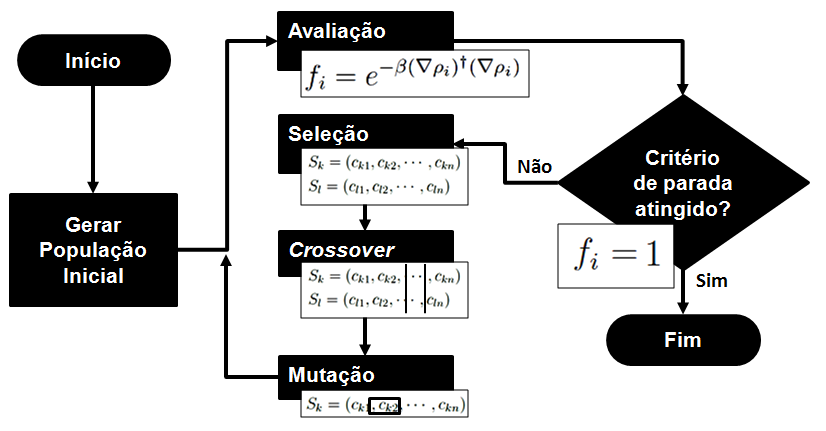
\includegraphics[width=0.90\textwidth]{figs/materiais_metodo/autovalores_com_ga/fluxo.png}
	\caption{Fluxo algoritmo genético}
	\label{fig:fluxo}
\end{figure}